% Options here are passed to the article class.
% Most common options: 10pt, 11pt, 12pt
\documentclass[10pt]{datasheet}

% Input encoding and typographical rules for English language
\usepackage[utf8]{inputenc}
\usepackage[english]{babel}
\usepackage[english]{isodate}

% tikz is used to draw images in this example, but you can
% also use \includegraphics{}.
\usepackage{graphicx}
\usepackage{float}
\usepackage{subcaption}

% These define global texts that are used in headers and titles.
\title{MG02: Minimum Hopper Box Merger}
\author{Floppydonkey}
\tags{merging, minimum-hopper, box-merger}
\date{25 December 2024}
\revision{Revision 1}
\begin{document}
\maketitle

\section{Features}

\begin{itemize}
\item{Uses only 3 hoppers per slice, the minimum required for a shulker box merger}
\item{Fully hopperlocked}
\item{Compact. 8x10x23 volume}
\item{Includes 8 merger slices to merge multiple boxes simultaneously}
\end{itemize}

\section{Applications}

\begin{itemize}
\item{Merging partial boxes in a dynamic sorting system}
\end{itemize}

\section{General Description}
The MG02 Minimum Hopper Box Merger is a device that can two partial shulker boxes into a full shulker box. The device is fully hopperlocked and uses the minimum number of hoppers required for a shulker box merger. Box comparison device for determining which box should be loaded/unloaded is not included.

\vfill\break

\begin{figure}[H]
    \centering
    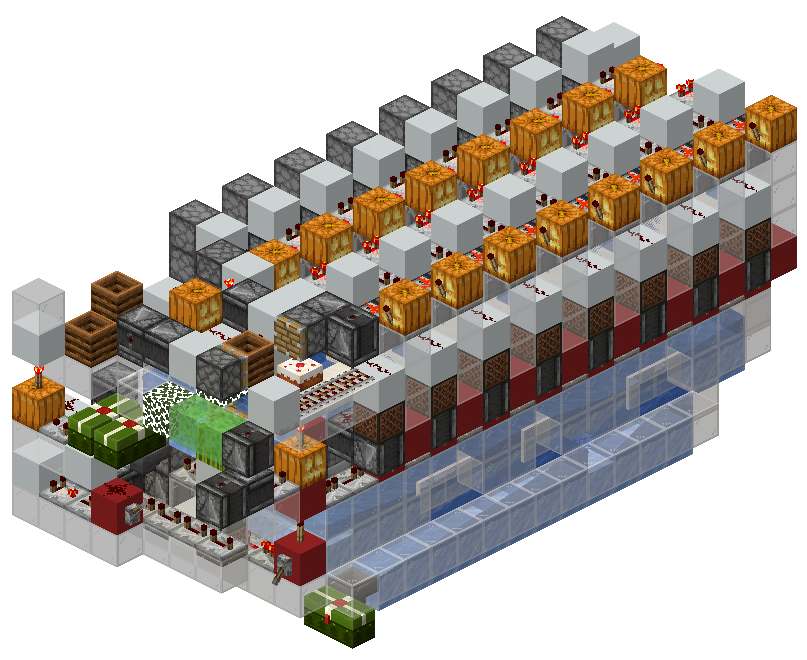
\includegraphics[width=0.48\textwidth]{area_render.png}
    \caption{\centering Minimum Hopper Box Merger}
\end{figure}

% For wide tables, a single column layout is better. It can be switched
% page-by-page.
\onecolumn

\section{Device Specifications}

\begin{table}[H]
    \caption{Inputs}
    \begin{tabularx}{\textwidth}{l | c | X}
        \thickhline
        \textbf{Name} & \textbf{Range} & \textbf{Description} \\
        \hline
        Loading input & Box & Partial box to be loaded during merging (right chest). \\
        \hline
        Unloading input & Box & Partial box to be unloaded during merging (left chest). \\
        \hline
        Hopperlocking input & 0-1 & Controls hopperlocking. \\
        \thickhline
\end{tabularx}
\end{table}

\begin{table}[H]
    \caption{Outputs}
    \begin{tabularx}{\textwidth}{l | c | X}
        \thickhline
        \textbf{Name} & \textbf{Range} & \textbf{Description} \\
        \hline
        Output boxes & Box & Merged shulker box output. \\
        \thickhline
\end{tabularx}
\end{table}

\begin{table}[H]
    \caption{Device Specifications}
    \begin{tabularx}{\textwidth}{l | c c c | c | X}
        \thickhline
        \textbf{Parameter} & \textbf{Min.} & \textbf{Typ.} & \textbf{Max.} &
        \textbf{Unit} & \textbf{Conditions} \\
        \hline
        MC Version & 1.16 & 1.17.1 & - & MCV & Latest version at time of writing: 1.21.4 \\
        \hline
        Dimensions & & 8 x 10 x 23 & & Blocks & \\
        \thickhline
\end{tabularx}
\end{table}
\section{Testing Data}
\begin{table}[H]
\caption{Executed Tests}
\begin{tabularx}{\textwidth}{l | X}
    \thickhline
    \textbf{Test} & \textbf{Result} \\
    \hline
    Merging test & Device was able to merge multiple boxes simultaneously. \\
    \thickhline
\end{tabularx}
\end{table}

\section{Download Information}
\begin{table}[H]
    \caption{Download Information}
    \begin{tabularx}{\textwidth}{l | l | l | X}
        \thickhline
        \textbf{Identifier} & \textbf{MC} & \textbf{File} & \textbf{Description} \\
        \hline
        MG02 & 1.17.1 & \href{https://github.com/Soontech-Annals/Archive/blob/8413f90a054b6c415703bae02badeba7541344f6/Archive/merging/MG02\%20Minimum\%20Hopper\%20Box\%20Merger/MG02\_Minimum\_Hopper\_Box\_Merger.litematic?raw=1}{MG02\_Minimum\_Hopper\_Box\_Merger.litematic} & Schematic of device. \\
        \hline
        \thickhline
    \end{tabularx}
\end{table}

\end{document}

